Alle im folgendem beschriebenen Eingaben (siehe \autoref{fig:instr_other_menu}) sind ausschließlich für den Super-User sichtbar. Der Einstieg erfolgt über den Punkt Administrator im Menü „Data-Input“.
\begin{figure}[H]
\centering
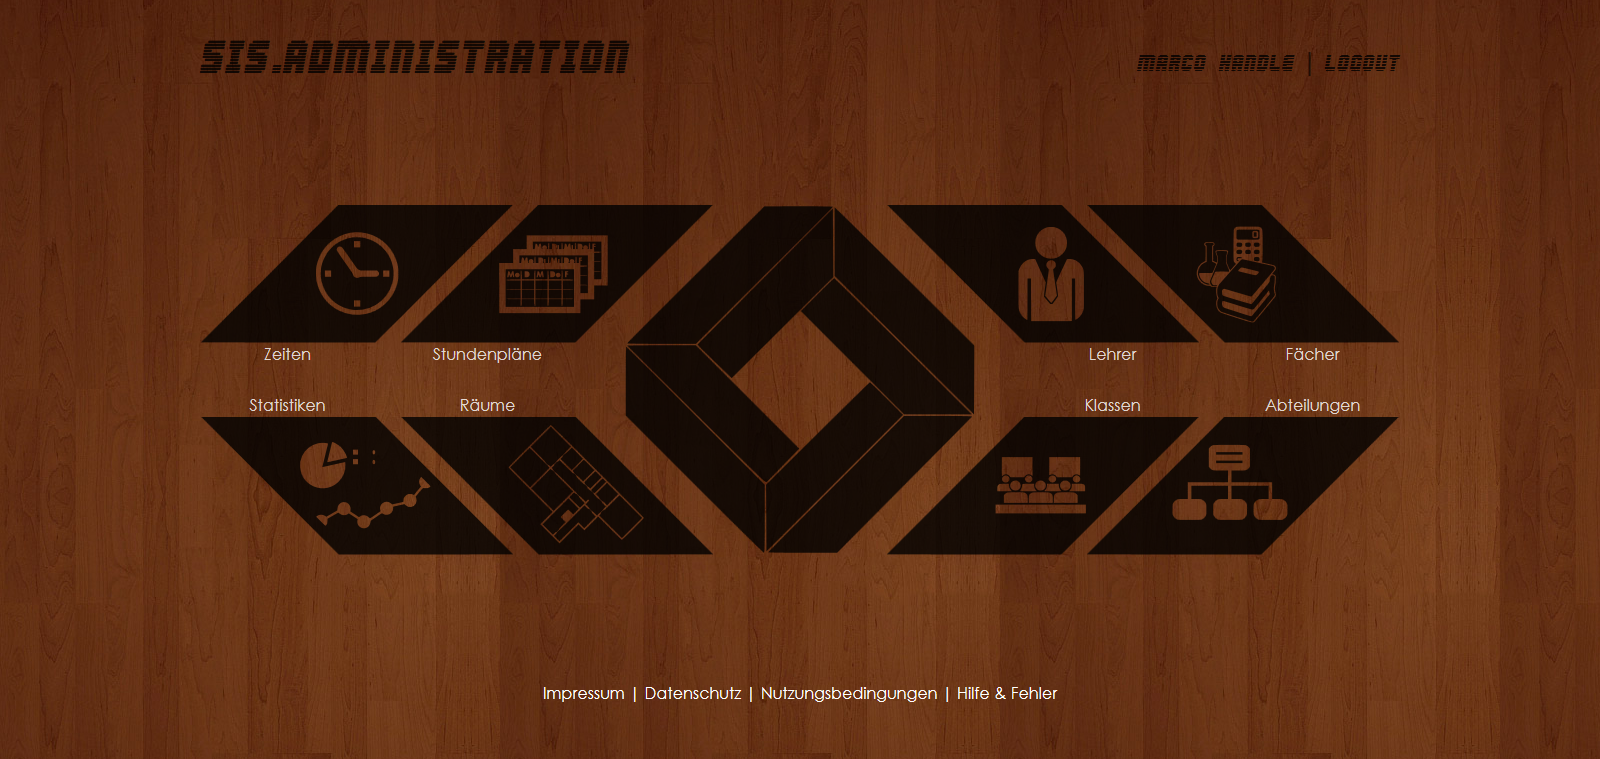
\includegraphics[keepaspectratio=true, width=17cm]{images/screenshots/admin_menu.png}
\caption{Administrationsmenü}
\label{fig:instr_other_menu}
\end{figure}
\subsection{Stunden}\label{sec:instr_other_hours}
Standardmäßig sind 16 Schulstunden mit der jeweiligen Start- und Endzeit für jeden Wochentag (Montag bis Freitag) angelegt (siehe \autoref{fig:instr_other_hours}). Über die Schaltfläche am linken bzw. rechten Seitenrand kann zwischen den Wochentagen gewechselt werden. Die Anzeige der Stunden wird entsprechend angepasst.\\
Die Änderungen können nun in den Eingabezeilen vorgenommen oder auch eine weitere Stunde angefügt werden. Alle Eingabefelder sind Pflichtfelder. Die Übernahme erfolgt mit der Schaltfläche Übernehmen in der jeweiligen Eingabezeile.\\
Aus Gründen der Datenkonsistenz der Stunden- und Supplierpläne ist das Löschen von Stunden nicht möglich.
\begin{figure}[H]
\centering
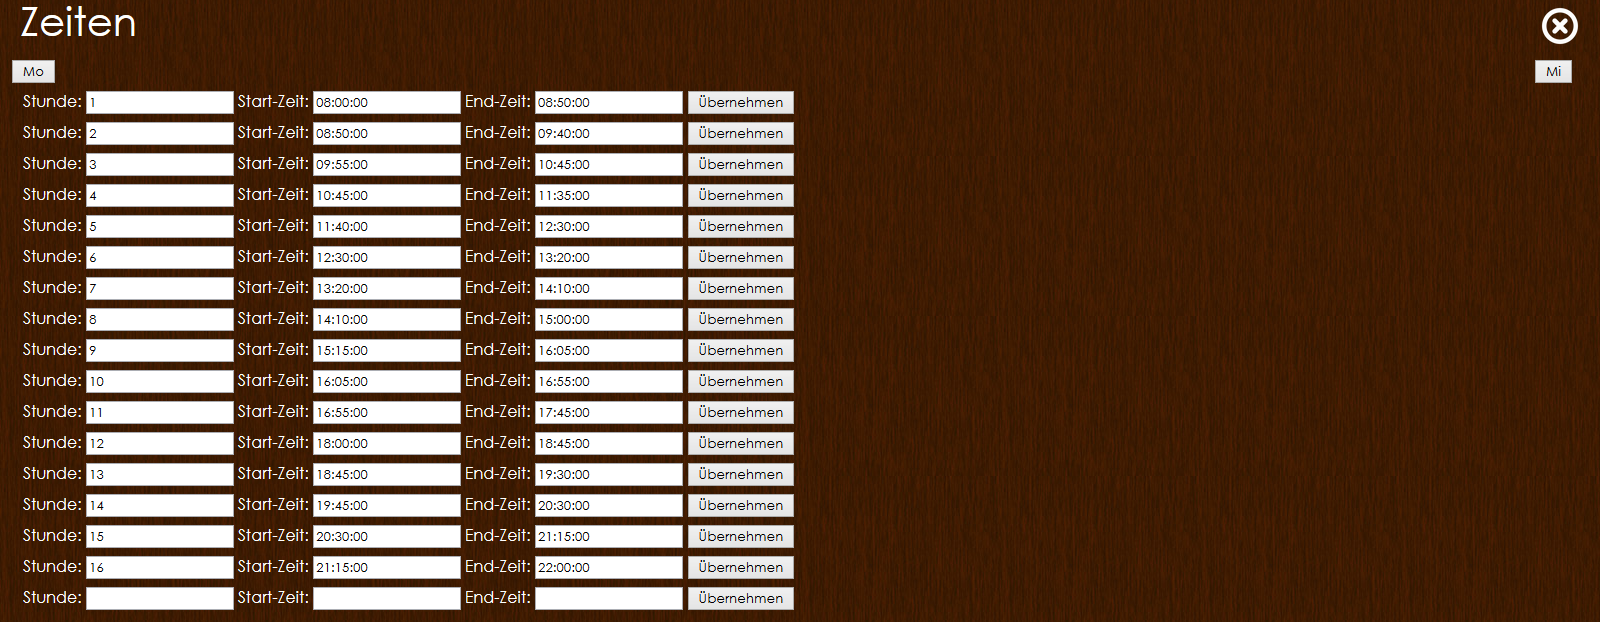
\includegraphics[keepaspectratio=true, width=17cm]{images/screenshots/hours_input.png}
\caption{Stunden bearbeiten}
\label{fig:instr_other_hours}
\end{figure}
\subsection{Stundenpläne}
Für die Erfassung eines Stundenplanes muss zuerst die Klasse (Listenfeld) und der Wochentag (Listenfeld) ausgewählt werden. Die Auswahl des Wochentages ist mit der Schaltfläche OK zu bestätigen (siehe \autoref{fig:instr_other_timetables_menu}). Ist bereits ein Stundenplan für den Tag vorhanden, wird dieser geladen (siehe \autoref{fig:instr_other_timetables_layout}). Über die Schaltfläche am linken bzw. rechten Seitenrand kann zwischen den Wochentagen gewechselt werden. Die Anzeige der Stunden wird entsprechend angepasst (siehe \autoref{fig:instr_other_timetables_day}).
Links oben werden die Klasse und der Wochentag angezeigt. Mit einem Klick auf die Klasse kehrt man ins Menü für die Auswahl der Klasse zurück (siehe \autoref{fig:instr_other_timetables_infos}).
\begin{figure}[H]
\centering
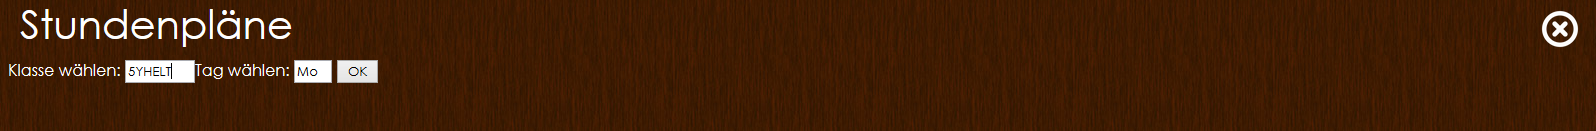
\includegraphics[keepaspectratio=true, width=17cm]{images/screenshots/timetables_input_menu.png}
\caption{Stundenplan auswählen}
\label{fig:instr_other_timetables_menu}
\end{figure}
\begin{figure}[H]
\centering
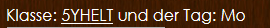
\includegraphics[keepaspectratio=true, width=6cm]{images/screenshots/timetables_input_infos.png}
\caption{Klasse und Tag}
\label{fig:instr_other_timetables_infos}
\end{figure}
\begin{figure}[H]
\centering
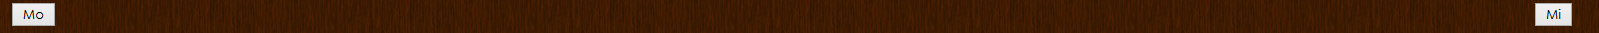
\includegraphics[keepaspectratio=true, width=17cm]{images/screenshots/timetables_input_day.png}
\caption{Tagauswahl}
\label{fig:instr_other_timetables_day}
\end{figure}
\begin{figure}[H]
\centering
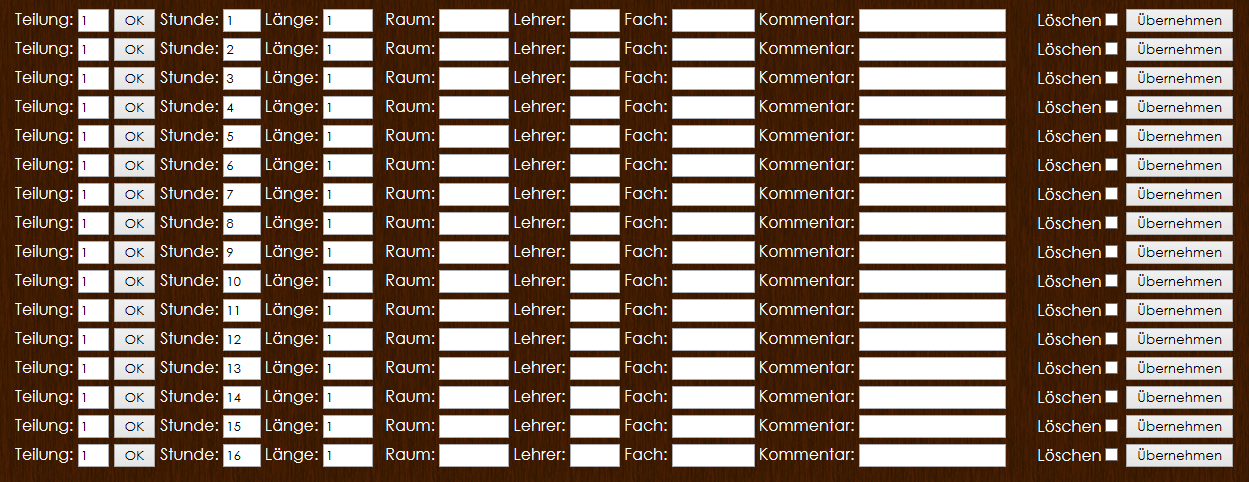
\includegraphics[keepaspectratio=true, width=17cm]{images/screenshots/timetables_input_layout.png}
\caption{Eingabemaske}
\label{fig:instr_other_timetables_layout}
\end{figure}
\subsubsection{Einstündiges Fach} \label{sec:instr_other_timetables_single}
Über die Standardeinstellung können Einzelstunden erfasst werden. In der entsprechenden Schulstunde sind der Lehrer und das Fach anzugeben.
\begin{table}[H]
\centering
\begin{tabular}{p{3 cm}p{10 cm}}
   \toprule
   \textbf{Eingabefeld} & \textbf{Typ} \\
   \midrule
          Teilung & \textbf{1} \newline nicht ändern \\
          \hline
          OK & Schaltfläche \\
          \hline
          Stunde & Schulstunde \newline Kann nicht geändert werden\\
          \hline
          Länge & \textbf{1} \newline Nicht ändern \\
          \hline
          Raum & Listenfeld - optional \\
          \hline
          \textbf{Lehrer} & Listenfeld - Pflichtfeld \\
		  \hline
          \textbf{Fach} & Listenfeld - Pflichtfeld.\\
          \hline
          Kommentar & Textfeld - optional \\
          \hline
          Löschen & Checkbox - \textbf{nicht gesetzt}\\
   \bottomrule
\end{tabular}
\caption{Eingabefelder Stundenplan}
\end{table}
Die Änderungen bzw. Ergänzungen sind mit der Schaltfläche Übernehmen in der jeweiligen Eingabezeile zu übernehmen (siehe \autoref{fig:instr_other_timetables_singleHour}).
\begin{figure}[H]
\centering
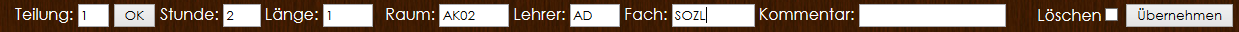
\includegraphics[keepaspectratio=true, width=17cm]{images/screenshots/timetables_input_singleHour.png}
\caption{Beispiel Einzelstunde}
\label{fig:instr_other_timetables_singleHour}
\end{figure}
\subsubsection{Mehrstündiges Fach}
Die Eingabe erfolgt analog zu jener im \autoref{sec:instr_other_timetables_single} beschriebenen. Es ist aber im Eingabefeld Länge die Anzahl der zusammenhängenden Schulstunden anzugeben. Wird nun in ein anderes Eingabefeld gewechselt, werden die nachfolgenden Eingabezeilen ausgeblendet, welche durch das mehrstündige Fach abgedeckt werden (siehe \autoref{fig:instr_other_timetables_multiHour}).\\
Wird zum Beispiel in der ersten Stunde ein Fach mit der Länge von 3 Stunden eingetragen, werden die Eingabezeilen der zweiten und dritte Stunde ausgeblendet.\\
Eingaben und Änderungen müssen jeweils durch das Drücken auf die Schaltfläche Übernehmen übernommen werden.
\begin{figure}[H]
\centering
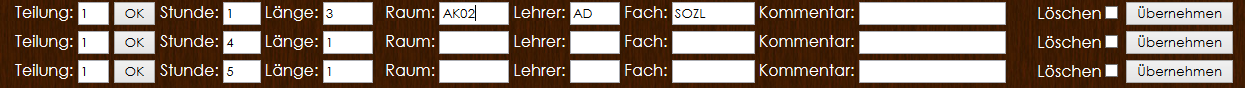
\includegraphics[keepaspectratio=true, width=17cm]{images/screenshots/timetables_input_multiHour.png}
\caption{Beispiel Mehrstündiger Unterricht}
\label{fig:instr_other_timetables_multiHour}
\end{figure}
\subsubsection{Teilung von Klassen}
Wird eine Klasse im Unterricht geteilt, ist dies über das Eingabefeld Teilung zu erfassen. Es ist zu beachten, dass die geteilten Fächer gleich lang sein müssen. Sind die geteilten Fächer ungleich lang, so ist der Rest der längeren Teilung als Einzelstunde zu erfassen. Eine Klasse kann maximal in 7 Teile geteilt werden.\\
Um eine Teilung erfassen zu können, ist im Eingabefeld Teilung die Anzahl der Teilungen einzugeben und mit der Schaltfläche OK zu bestätigen. Anschließend erscheinen weitere Eingabezeilen (siehe \autoref{fig:instr_other_timetables_divide7}).\\
Die Eingabe erfolgt sinngemäß wie die Erfassung eines mehrstündigen Fachs. Jede einzelne Eingabezeile der Teilung ist mit der Schaltfläche Übernehmen zu bestätigen.
\begin{figure}[H]
\centering
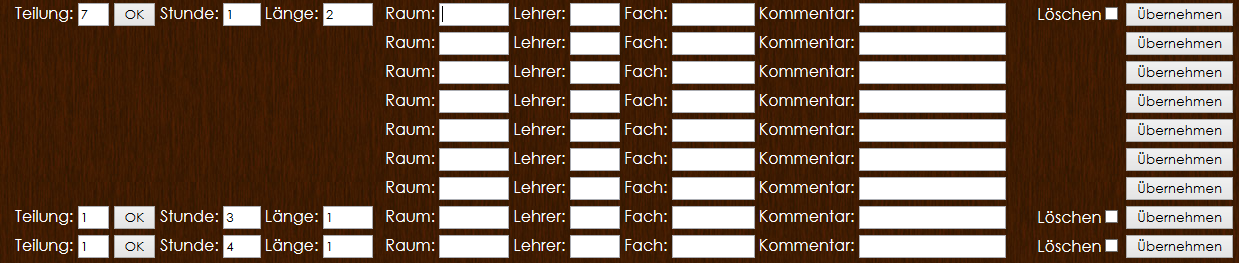
\includegraphics[keepaspectratio=true, width=17cm]{images/screenshots/timetables_input_divide7.png}
\caption{Beispiel Teilungen}
\label{fig:instr_other_timetables_divide7}
\end{figure}
Jede eigene Zeile muss mit Übernehmen bestätigt werden. Gelöscht kann jedoch nur ein ganzer Block werden. Dies muss mit einem Haken bei Löschen und anschließendem Klicken auf Übernehmen erfolgen.
\subsubsection{Löschen von Unterrichtsstunden}
Das Löschen von Einträgen kann einzeln über die Checkbox Löschen vorgenommen werden. Der Stundenplan eines Tages kann über die Schaltfläche \enquote{Stundenplan löschen} \textbf{unwiderruflich} gelöscht werden (siehe \autoref{fig:instr_other_timetables_delete}).
\begin{figure}[H]
\centering
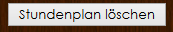
\includegraphics[keepaspectratio=true, width=5cm]{images/screenshots/timetables_input_delete.png}
\caption{Löschen}
\label{fig:instr_other_timetables_delete}
\end{figure}
\subsection{Lehrer}
Dieser Punkt ist dazu da, dass man Lehrer bearbeiten und hinzufügen kann. Auch hier ist es nicht möglich Lehrer zu löschen, da es wie bei Stunden zu großen Problemen kommen kann. (siehe \gref{sec:instr_other_hidden})\\
Im Feld Name muss der vollständige Name des Lehrers eingegeben werden, im Feld Kürzel wird das Lehrer-Kürzel eingetragen, im Feld Kurzname muss ein verkürzter Name eingegeben werden, dieser wird zum Beispiel bei den Supplierungen am Display angezeigt. Im Feld Stammabteilung kann eine Abteilung eingegeben werden, dies ist jedoch optional, da nicht jeder Lehrer eine Stammabteilung hat. Wie schon erwähnt ist der Haken für unsichtbar zum stilllegen eines Lehrers gut. (Eingabemaske siehe \autoref{fig:instr_other_teacher}) Sollen vorhandene Daten geändert werden, so kann man den vorhandenen Lehrer abändern und mit Übernehmen speichern.
\begin{figure}[H]
\centering
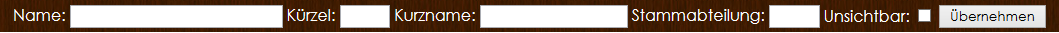
\includegraphics[keepaspectratio=true, width=17cm]{images/screenshots/teachers_input.png}
\caption{Eingabemaske Lehrer}
\label{fig:instr_other_teacher}
\end{figure}
\subsection{Fächer}
Über diese Eingabemaske werden Lehrereinträge bearbeitet und hinzugefügt (siehe \autoref{fig:instr_other_subjects}). Aus Gründen der Datenkonsistenz der Stunden- und Supplierpläne ist das Löschen von Lehrern nicht möglich.
\begin{table}[H]
\centering
\begin{tabular}{p{3 cm}p{10 cm}}
   \toprule
   \textbf{Eingabefeld} & \textbf{Typ} \\
   \midrule
          \textbf{Name} & Textfeld - Pflichtfeld \newline vollständiger Name \\
          \hline
          \textbf{Kürzel} & Textfeld - Pflichtfeld \newline Lehrer-Kürzel \\
          \hline
          \textbf{Kurzname} & Textfeld - Pflichtfeld \newline Kurzname für die Anzeige am Display \\
          \hline
          Stammabteilung & Textfeld - optional \\
          \hline
          Unsichtbar & Checkbox \\
   \bottomrule
\end{tabular}
\caption{Eingabefelder Fächer}
\end{table}
Wird die Checkbox Unsichtbar bei einem Lehrer gesetzt, wird dieser in den Listenfelder nicht mehr angezeigt. (siehe \gref{sec:instr_other_hidden})\\
Änderungen und Ergänzungen sind über die Schaltfläche Übernehmen in den Eingabezeilen zu bestätigen.
\begin{figure}[H]
\centering
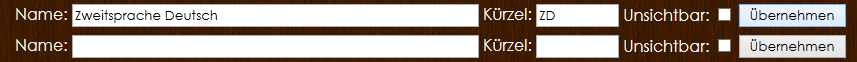
\includegraphics[keepaspectratio=true, width=17cm]{images/screenshots/subjects_input.png}
\caption{Eingabemaske Fächer}
\label{fig:instr_other_subjects}
\end{figure}
\subsection{Statistiken}
Um die Akzeptanz der Anwendung beurteilen zu können, wurde ein Statistikmodul implementiert, obwohl dies im vorgegebenen Pflichtenheft nicht vorgesehen ist. Es werden deshalb unter anderem anonymisiert die Zugriffe auf die verschiedenen Seiten, von welchen Endgeräten die Zugriffe erfolgen, welche Schulstufen, etc. registriert und in Grafiken ausgewertet.
\begin{figure}[H]
\centering
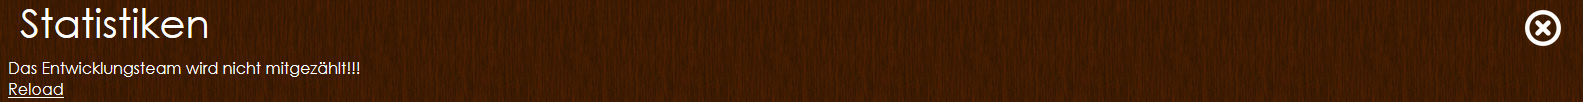
\includegraphics[keepaspectratio=true, width=17cm]{images/screenshots/statistics_header.png}
\caption{Statistiken Reload}
\label{fig:instr_other_statistics_header}
\end{figure}
\subsubsection{Browser PC}
In dieser Statistik sind die Browser der Geräte dargestellt, welche die PC Seiten aufrufen. (siehe \autoref{fig:instr_other_statistics_browser_PC})
\begin{figure}[H]
\centering
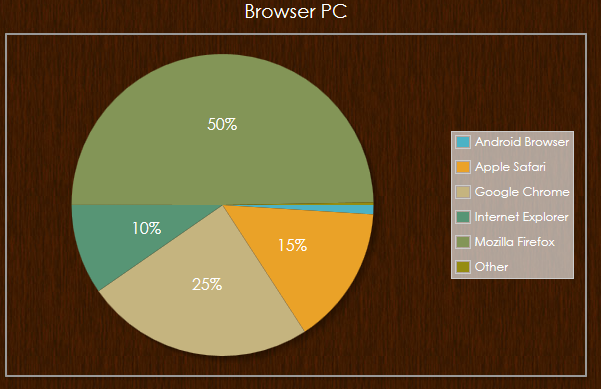
\includegraphics[keepaspectratio=true, width=8cm]{images/screenshots/statistics_browser_PC.png}
\caption{Browser PC}
\label{fig:instr_other_statistics_browser_PC}
\end{figure}
\subsubsection{Geräte PC}
In dieser Statistik sind die Geräte bzw. Betriebssysteme der Geräte dargestellt, welche die PC Seiten aufrufen. (siehe \autoref{fig:instr_other_statistics_os_PC})
\begin{figure}[H]
\centering
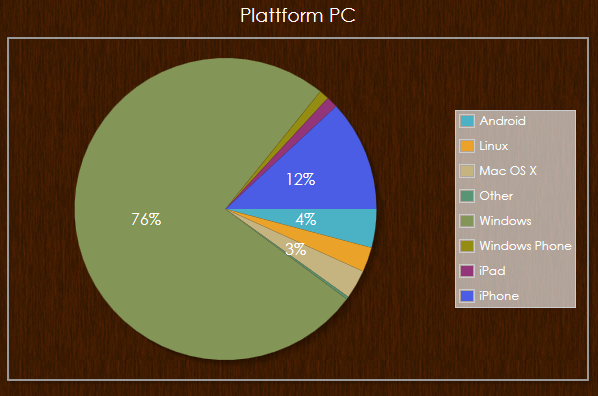
\includegraphics[keepaspectratio=true, width=8cm]{images/screenshots/statistics_os_PC.png}
\caption{Geräte PC}
\label{fig:instr_other_statistics_os_PC}
\end{figure}
\subsubsection{Browser Mobil}
In dieser Statistik sind die Browser der Geräte dargestellt, welche die App aufrufen. (siehe \autoref{fig:instr_other_statistics_browser_Mob})
\begin{figure}[H]
\centering
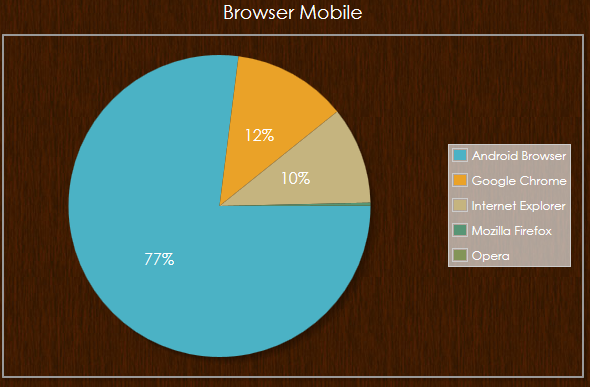
\includegraphics[keepaspectratio=true, width=8cm]{images/screenshots/statistics_browser_Mob.png}
\caption{Browser Mobil}
\label{fig:instr_other_statistics_browser_Mob}
\end{figure}
\subsubsection{Geräte Mobil}
In dieser Statistik sind die Geräte bzw. Betriebssysteme der Geräte dargestellt, welche die App Seiten aufrufen. (siehe \autoref{fig:instr_other_statistics_os_Mob})
\begin{figure}[H]
\centering
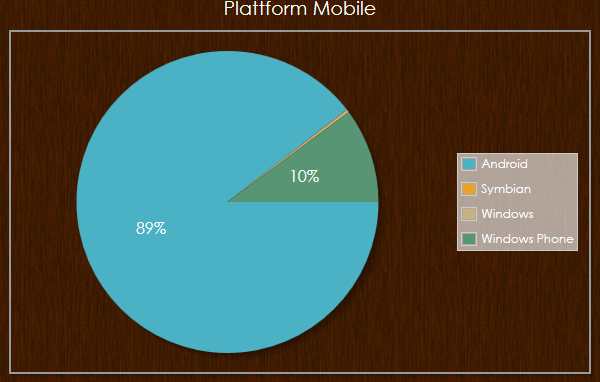
\includegraphics[keepaspectratio=true, width=8cm]{images/screenshots/statistics_os_Mob.png}
\caption{Browser PC}
\label{fig:instr_other_statistics_os_Mob}
\end{figure}
\subsubsection{Nutzer}
In dieser Statistik sind die Nutzer nach den Schulstufen und nach den Lehrern aufgeteilt. Hier kann herausgelesen werden welcher Jahrgang den Service am häufigsten nutzt. (siehe \autoref{fig:instr_other_statistics_user})
\begin{figure}[H]
\centering
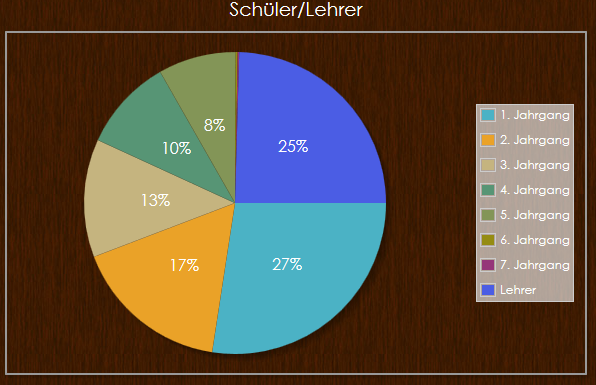
\includegraphics[keepaspectratio=true, width=8cm]{images/screenshots/statistics_user.png}
\caption{Nutzer}
\label{fig:instr_other_statistics_user}
\end{figure}
\subsubsection{Abteilungen}
In dieser Statistik werden die Nutzer nach ihrer Abteilung aufgeteilt, dabei werden nur die Schüler gezählt. Hier kann herausgelesen werden welche Abteilung den Service am häufigsten nutzt. (siehe \autoref{fig:instr_other_statistics_sections})
\begin{figure}[H]
\centering
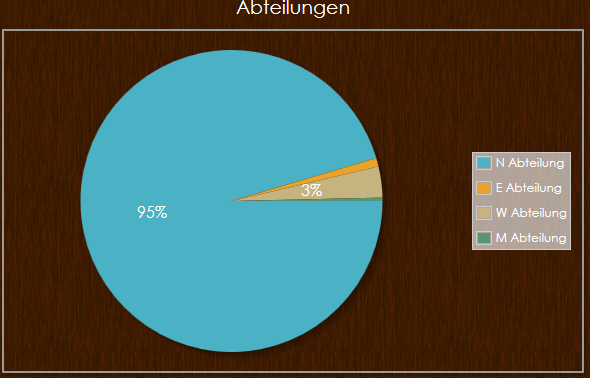
\includegraphics[keepaspectratio=true, width=8cm]{images/screenshots/statistics_sections.png}
\caption{Abteilungen}
\label{fig:instr_other_statistics_sections}
\end{figure}
\subsubsection{Supplierungen}
In dieser Statistik wird dargestellt welche Seite die User am häufigsten benützen, um die Supplierungen anzusehen. Dabei wird der Supplierplan im Web, Supplierplan in der App , der modifizierte Stundenplan in der App und der modifizierte Stundenplan im Web analysiert. (siehe \autoref{fig:instr_other_statistics_substitudes})
\begin{figure}[H]
\centering
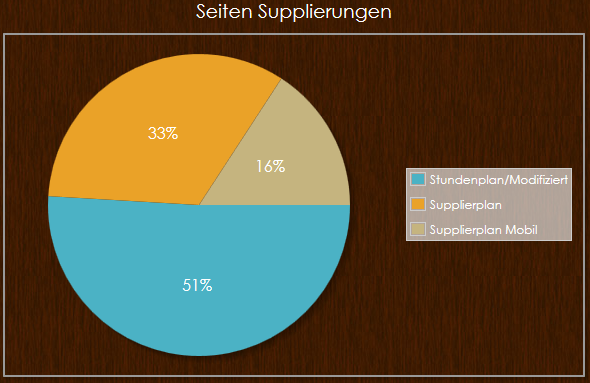
\includegraphics[keepaspectratio=true, width=8cm]{images/screenshots/statistics_substitudes.png}
\caption{Supplierungen}
\label{fig:instr_other_statistics_substitudes}
\end{figure}
\subsubsection{App/Web}
In dieser Statistik wird die App und die Webseite gegenübergestellt und man kann auslesen welcher Dienst öfters genutzt wird. (siehe \autoref{fig:instr_other_statistics_app_web})
\begin{figure}[H]
\centering
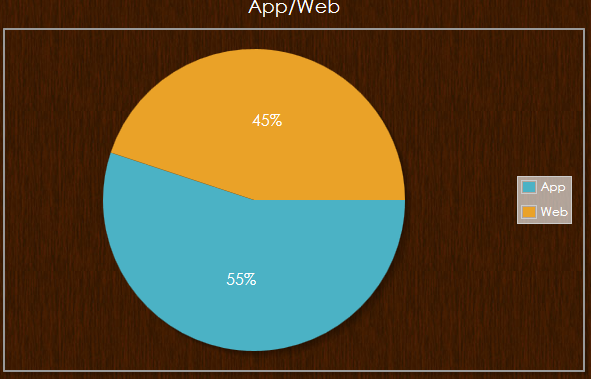
\includegraphics[keepaspectratio=true, width=8cm]{images/screenshots/statistics_app_web.png}
\caption{App/Web}
\label{fig:instr_other_statistics_app_web}
\end{figure}
\subsubsection{Seiten Web}
In dieser Statistik wird dargestellt welche Seiten die User auf der Webseite am häufigsten besuchen. (siehe \autoref{fig:instr_other_statistics_sites_web})
\begin{figure}[H]
\centering
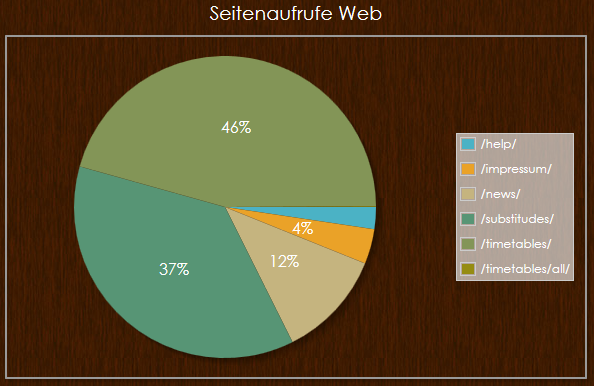
\includegraphics[keepaspectratio=true, width=8cm]{images/screenshots/statistics_sites_web.png}
\caption{Seiten Web}
\label{fig:instr_other_statistics_sites_web}
\end{figure}
\subsubsection{Seiten App}
In dieser Statistik wird dargestellt welche Seiten die User in der App am häufigsten besuchen. (siehe \autoref{fig:instr_other_statistics_sites_app})
\begin{figure}[H]
\centering
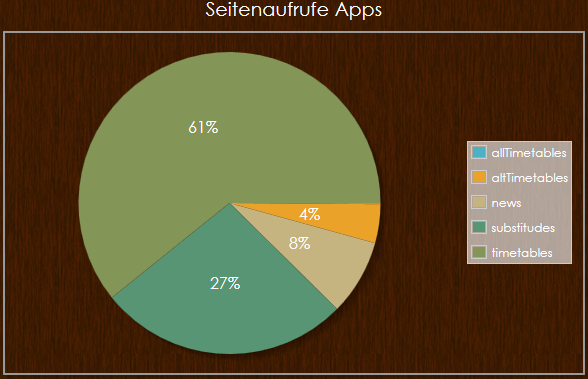
\includegraphics[keepaspectratio=true, width=8cm]{images/screenshots/statistics_sites_app.png}
\caption{Seiten App}
\label{fig:instr_other_statistics_sites_app}
\end{figure}
\subsubsection{Seitenaufrufe Stunden}
In dieser Statistik wird dargestellt, wie viele Seitenaufrufe im Durchschnitt in welcher Stunde am Tag auftreten. (siehe \autoref{fig:instr_other_statistics_view_day})
\begin{figure}[H]
\centering
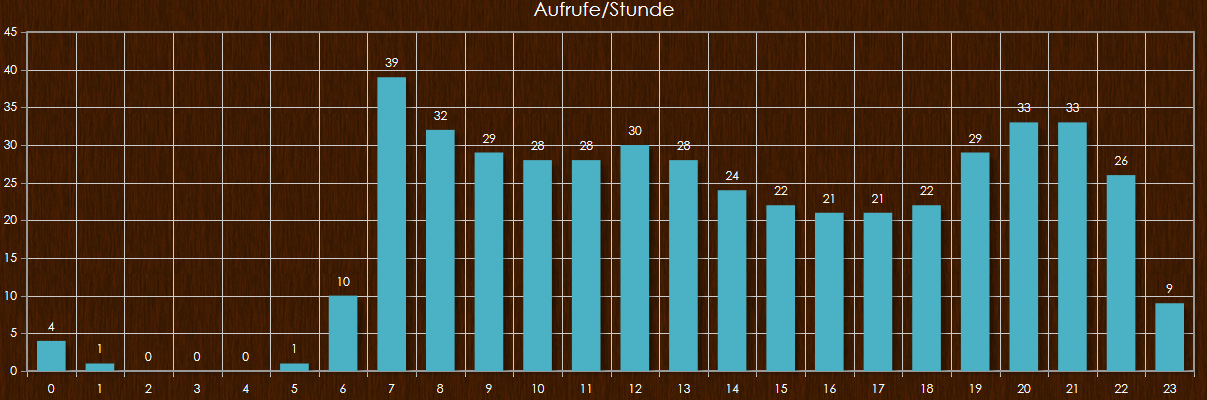
\includegraphics[keepaspectratio=true, width=17cm]{images/screenshots/statistics_views_hour.png}
\caption{Seitenaufrufe Stunden}
\label{fig:instr_other_statistics_view_day}
\end{figure}
\subsubsection{Seitenaufrufe täglich}
In dieser Statistik wird dargestellt, wie viele Seitenaufrufe jeden Tag verursacht werden. (siehe \autoref{fig:instr_other_statistics_views_day}) Hier kann auch, um bei vielen Tagen sich einen Überblick zu beschaffen, hineingezoomt werden. Dies macht man in dem man mit der linken Maustaste ein gewünschtes Fenster aufzieht. Heraus zoomen kann mit einem doppelten rechts Klick gemacht werden. (siehe \autoref{fig:instr_other_statistics_views_day_zoom})
\begin{figure}[H]
\centering
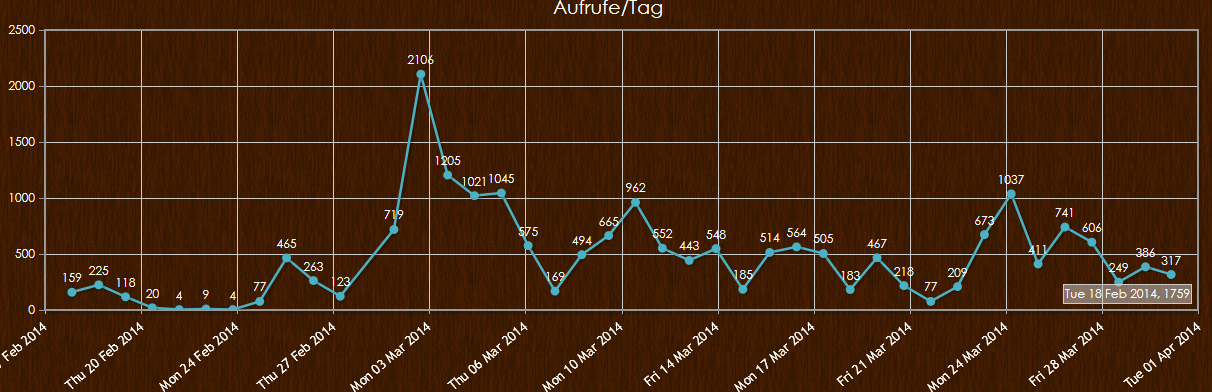
\includegraphics[keepaspectratio=true, width=17cm]{images/screenshots/statistics_views_day.png}
\caption{Seitenaufrufe täglich}
\label{fig:instr_other_statistics_views_day}
\end{figure}
\begin{figure}[H]
\centering
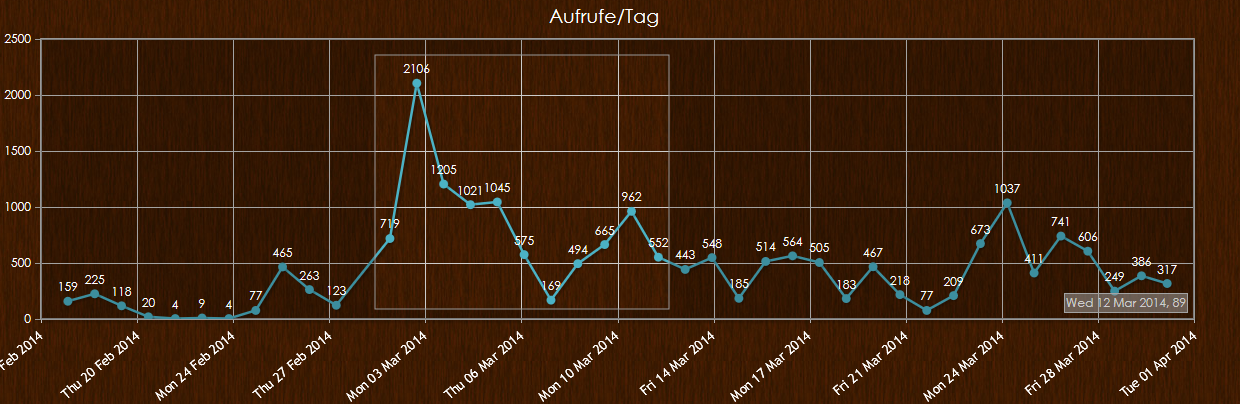
\includegraphics[keepaspectratio=true, width=17cm]{images/screenshots/statistics_views_day_zoom.png}
\caption{Seitenaufrufe täglich zoomen}
\label{fig:instr_other_statistics_views_day_zoom}
\end{figure}
\subsection{Räume}
Über diese Eingabemaske werden Räume bearbeitet und hinzugefügt (siehe \autoref{fig:instr_other_room_input}). Aus Gründen der Datenkonsistenz der Stunden- und Supplierpläne ist das Löschen von Räumen nicht möglich.
\begin{table}[H]
\centering
\begin{tabular}{p{3 cm}p{10 cm}}
   \toprule
   \textbf{Eingabefeld} & \textbf{Typ} \\
   \midrule
          \textbf{Name} & Textfeld - Pflichtfeld \newline Name des Raumes \\
          \hline
          Zuständiger Lehrer & Listenfeld - optional \newline Verantwortlicher Lehrer für den Raum\\
   \bottomrule
\end{tabular}
\caption{Eingabefelder Räume}
\end{table}
Änderungen und Ergänzungen sind über die Schaltfläche Übernehmen in den Eingabezeilen zu bestätigen.
\begin{figure}[H]
\centering
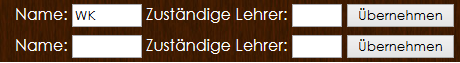
\includegraphics[keepaspectratio=true, width=10cm]{images/screenshots/rooms_input.png}
\caption{Eingabemaske Räume}
\label{fig:instr_other_room_input}
\end{figure}
\subsection{Klassen}
Über diese Eingabemaske werden Klassen bearbeitet und hinzugefügt (siehe \autoref{fig:instr_other_classes_input}). Aus Gründen der Datenkonsistenz der Stunden- und Supplierpläne ist das Löschen von Klassen nicht möglich. Jedoch können Klassen als unsichtbar gekennzeichnet werden (siehe \gref{sec:instr_other_hidden}).
\begin{table}[H]
\centering
\begin{tabular}{p{3 cm}p{10 cm}}
   \toprule
   \textbf{Eingabefeld} & \textbf{Typ} \\
   \midrule
          \textbf{Name} & Textfeld - Pflichtfeld \newline Name der Klasse \\
          \hline
          \textbf{Abteilung} & Listenfeld - Pflichtfeld \\
          \hline
          Klassenvorstand & Listenfeld - optional \\
          \hline
          Stammklasse & Textfeld - optional \newline Zugeordneter Klassenraum \\
          \hline
          Unsichtbar & Checkbox \\
   \bottomrule
\end{tabular}
\caption{Eingabe Klassen}
\end{table}
Wanderklassen kann der Raum WK als Scheinklassenraum zugewiesen werden. Wird die Checkbox Unsichtbar bei einer Klasse gesetzt, wird diese in den Listenfelder nicht mehr angezeigt.\\
Änderungen und Ergänzungen sind über die Schaltfläche Übernehmen in den Eingabezeilen zu bestätigen.
\begin{figure}[H]
\centering
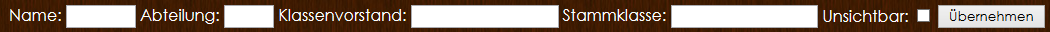
\includegraphics[keepaspectratio=true, width=17cm]{images/screenshots/classes_input.png}
\caption{Eingabemaske Klassen}
\label{fig:instr_other_classes_input}
\end{figure}
\subsection{Abteilungen}
Über diese Eingabemaske werden Abteilungen bearbeitet und hinzugefügt (siehe \autoref{fig:instr_other_sections_input}). Aus Gründen der Datenkonsistenz der Stunden- und Supplierpläne ist das Löschen von Abteilungen nicht möglich.
\begin{table}[H]
\centering
\begin{tabular}{p{3 cm}p{10 cm}}
   \toprule
   \textbf{Eingabefeld} & \textbf{Typ} \\
   \midrule
          \textbf{Name} & Textfeld - Pflichtfeld \newline Vollständiger Bezeichnung der Abteilung \\
          \hline
          \textbf{Kürzel} & Listenfeld - Pflichtfeld \\
          \hline
          \textbf{Abteilungsleiter} & Listenfeld - Pflichtfeld \\
   \bottomrule
\end{tabular}
\caption{Eingabe Abteilungen}
\end{table}
\begin{figure}[H]
\centering
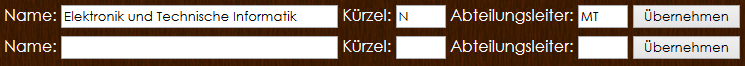
\includegraphics[keepaspectratio=true, width=17cm]{images/screenshots/sections_input.png}
\caption{Eingabemaske Abteilungen}
\label{fig:instr_other_sections_input}
\end{figure}
\subsection{Unsichtbar}\label{sec:instr_other_hidden}
Aus Sicherheitsgründen und Gründen der Datenkonsistenz dürfen manche Daten nicht gelöscht werden. Das Löschen ist nur dort möglich, wo explizit eine Checkbox Löschen vorhanden ist.\\
Um dennoch unnötige Einträge in den Listenfeldern zu vermeiden, können über die Checkbox Unsichtbar Einträge deaktiviert werden. Über die gleiche Funktion können diese Einträge dann wenn notwendig wieder aktiviert werden.
\subsection{DropDown-Menüs}
In zahlreichen Eingabefeldern sind Listen der zulässigen Eingaben hinterlegt, welche bei Beginn der Eingabe angezeigt werden. In Abhängigkeit der eingegebenen Zeichen wird die angezeigte Liste eingeschränkt. Ist die angezeigte Liste leer, so wurde kein übereinstimmender Eintrag gefunden und liegt wahrscheinlich eine Fehleingabe vor.